\documentclass[journal]{IEEEtran}

\usepackage[T1]{fontenc}
\usepackage[utf8]{inputenc}
\usepackage{amsmath,amssymb}
\usepackage{graphicx}
\usepackage{booktabs}
\usepackage{array}
\usepackage{cite}
\usepackage[hidelinks]{hyperref}
\graphicspath{{figures/}}

\begin{document}

\title{A Longitudinal EEG Aging Manifold Derived From Resting-State Spectral Dynamics Across the Adult Lifespan}

\author{Antonio Pereira,~\IEEEmembership{Member,~IEEE}}

\markboth{IEEE Journal of Biomedical and Health Informatics}%
{Pereira: A Longitudinal EEG Aging Manifold}

\maketitle

\begin{abstract}
Resting-state electroencephalography (EEG) provides a non-invasive and scalable measure of adult brain function, but most brain-aging studies reduce electrophysiological aging to cross-sectional age prediction. Here, we derive and validate a low-dimensional EEG aging manifold from 64-channel resting-state EEG recordings across the adult lifespan. We analyzed OpenNeuro ds005385, containing baseline eyes-closed EEG from 608 healthy adults aged 20--70 years and five-year follow-up recordings from 208 participants. Spectral features were extracted from global and regional EEG power in canonical frequency bands, including absolute power, relative power, theta/alpha and beta/alpha ratios, individual alpha frequency, and aperiodic spectral slope. A ridge-regression EEG brain-age model predicted chronological age with mean absolute error (MAE) of 9.46 years, correlation $r=0.611$, and $R^2=0.371$. Age-associated spectral structure was dominated by increasing relative beta power and decreasing high-alpha power. Principal component analysis showed that the first ten components explained 91.68\% of EEG feature variance, and a two-dimensional aging trajectory based on PC1 and PC4 was significantly associated with chronological age ($\rho=0.344$, $p=2.73\times10^{-18}$). In the longitudinal subset, participants moved significantly forward along the inferred EEG aging trajectory from session 1 to session 2 (mean $\Delta T=0.403$, median $\Delta T=0.522$, Wilcoxon $p=0.0020$), whereas orthogonal deviation from the trajectory did not change ($p=0.622$). Baseline trajectory position predicted future trajectory change ($\rho=-0.280$, $p=4.09\times10^{-5}$), whereas chronological age did not ($\rho=-0.018$, $p=0.795$). These results identify a stable electrophysiological aging manifold whose longitudinal dynamics are not reducible to chronological age.
\end{abstract}

\begin{IEEEkeywords}
EEG, brain age, aging, resting-state EEG, longitudinal biomarkers, manifold learning, spectral power, alpha rhythm, beta rhythm, biomedical informatics.
\end{IEEEkeywords}

\section{Introduction}

Population aging increases the need for scalable biomarkers capable of quantifying individual differences in brain function across adulthood. Magnetic resonance imaging has provided a mature framework for brain-age estimation, in which multivariate brain features are used to predict chronological age and the residual between predicted and observed age is interpreted as a marker of brain health \cite{franke2010estimating,cole2017predicting,bashyam2020mri,cole2020multimodality}. However, MRI-based biomarkers are expensive, immobile, and poorly suited for repeated large-scale assessment. Resting-state EEG offers a complementary route because it is inexpensive, temporally precise, repeatable, and sensitive to neural oscillatory changes across the lifespan \cite{dustman1993eeg,klimesch1999eeg,voytek2015age,donoghue2020parameterizing}.

Adult aging is accompanied by systematic changes in resting EEG spectra. Alpha rhythms, especially posterior and high-alpha activity, show age-related changes, while beta-band and aperiodic spectral properties also vary with age \cite{dustman1993eeg,haegens2014alpha,mierau2017state,voytek2015age,donoghue2020parameterizing}. These effects are not isolated to single electrodes or narrow bands. Rather, they form coordinated multivariate patterns over scalp regions and frequency bands. Therefore, electrophysiological aging should be modeled as a trajectory in a structured feature space, not only as a scalar regression problem.

Brain-age models are useful for prediction, but they do not by themselves identify the geometry of aging. A model may predict age while obscuring whether aging corresponds to motion along a coherent low-dimensional trajectory or to diffuse changes across many independent features. Brain-age gaps are also affected by age-level bias, a regression-to-the-mean effect in which younger participants tend to be predicted as older and older participants tend to be predicted as younger \cite{le2018nonlinear,smith2020brain,liang2023age}. These issues motivate a representation that separates trajectory position from deviation around that trajectory.

In this study, we derive a longitudinal EEG aging manifold from resting-state EEG. The central hypothesis is that adult EEG aging is expressed as movement along a low-dimensional spectral trajectory, and that this trajectory has longitudinal validity. We test four predictions. First, resting-state EEG spectral features predict chronological age. Second, age-related EEG variation is concentrated in a low-dimensional latent space. Third, participants with repeated recordings move along the inferred aging trajectory between baseline and follow-up. Fourth, baseline trajectory position predicts future movement along the manifold independently of chronological age.

\section{Dataset}

We analyzed OpenNeuro dataset ds005385, a resting-state EEG dataset acquired across the adult lifespan with follow-up measurements \cite{getzmann2024resting,openneuro_ds005385}. The dataset contains 64-channel resting-state EEG recordings from 608 adults aged 20--70 years, with eyes-open and eyes-closed recordings before and after a two-hour cognitive activity block. A follow-up session approximately five years later is available for 208 participants. The present analysis used eyes-closed, pre-task recordings as the baseline state. Baseline analyses included all 608 participants. Longitudinal analyses included the 208 participants with session-2 eyes-closed pre-task recordings. The data are organized according to the Brain Imaging Data Structure and EEG-BIDS conventions \cite{gorgolewski2016bids,pernet2019eegbids}.

\section{Methods}

\subsection{EEG File Selection and Channel Inclusion}

EDF files were selected if their filenames indicated eyes-closed resting-state EEG acquired before the cognitive activity block. Baseline analyses used files matching session 1, eyes closed, acquisition pre. Longitudinal analyses used the corresponding session-2, eyes-closed, acquisition-pre recordings. Each EDF file was parsed with MNE-Python \cite{gramfort2013meg}. Channels marked as EEG channels by the file metadata were retained; non-EEG channels were excluded. Channel names were matched case-insensitively after removal of non-alphanumeric separators. Files were required to contain at least one valid EEG channel in each regional group used for regional features. In the analyzed baseline and longitudinal subsets, all selected files were processed successfully.

No independent-component analysis, automated bad-channel interpolation, or epoch-level artifact rejection was applied. This choice preserves a fixed, reproducible, file-level feature extraction pipeline and avoids introducing subject-specific preprocessing decisions into the longitudinal trajectory analysis. Recordings that could not be loaded or did not contain the required task/acquisition combination were logged as failures; no failures occurred in the 608 baseline files or the 208 session-2 follow-up files used in the reported analyses.

\subsection{EEG Preprocessing}

Signals were resampled to 250 Hz, band-pass filtered from 1 to 45 Hz, notch filtered at 50 Hz, and re-referenced to the average reference. Power spectra were estimated using Welch's method with 512-point FFT windows and 50\% overlap \cite{welch1967use,cohen2014analyzing}. Let $x_{ic}(t)$ denote the preprocessed EEG signal for participant $i$ and channel $c$. The power spectral density was estimated as

\begin{equation}
P_{ic}(f)=\mathrm{Welch}\{x_{ic}(t)\}.
\end{equation}

Canonical frequency bands were defined as delta (1--4 Hz), theta (4--8 Hz), alpha (8--13 Hz), low alpha (8--10 Hz), high alpha (10--13 Hz), beta (13--30 Hz), and gamma (30--45 Hz). These bands were used for all global and regional feature calculations.

\subsection{Regional Spectral Features}

Channels were grouped into frontal, central, temporal, parietal, and occipital regions using standard scalp topography. The frontal group included Fp, AF, and F channels; the central group included FC, C, and CP channels; the temporal group included FT, T, TP, and lateral temporal-parietal channels; the parietal group included P and PO channels; and the occipital group included O and posterior occipital-parietal channels. For each file, the regional channel set was the intersection between the region definition and the channels present in the recording. Global features used all retained EEG channels. This rule allows regional features to remain well defined under minor channel-name variation.

For a region $r$ with channel set $\mathcal{C}_r$ and frequency band $b=[f_1,f_2]$, absolute regional power was computed as

\begin{equation}
A_{irb}=\sum_{c\in\mathcal{C}_r}\sum_{f\in b} P_{ic}(f).
\end{equation}

Relative power was computed as

\begin{equation}
R_{irb}=\frac{A_{irb}}{\sum_{c\in\mathcal{C}_r}\sum_{f=1}^{45}P_{ic}(f)}.
\end{equation}

Global features were computed analogously using all EEG channels. Ratio features included

\begin{equation}
Q^{\theta/\alpha}_{i}=\frac{A_{i,\theta}}{A_{i,\alpha}+\epsilon},
\end{equation}

and

\begin{equation}
Q^{\beta/\alpha}_{i}=\frac{A_{i,\beta}}{A_{i,\alpha}+\epsilon},
\end{equation}

with $\epsilon=10^{-30}$ for numerical stability. Individual alpha frequency was defined as the frequency of maximal mean power in the 8--13 Hz range, estimated globally and in posterior regions. Aperiodic slope was estimated by linear regression in log-log spectral coordinates outside the alpha band, following the separation of periodic and aperiodic spectral structure proposed in modern spectral parameterization work \cite{voytek2015age,donoghue2020parameterizing}:

\begin{equation}
\log_{10} P_i(f) = \alpha_i + \gamma_i \log_{10} f + \varepsilon_i,
\end{equation}

where $\gamma_i$ is the aperiodic slope and $\alpha_i$ is the intercept.

The final predictor matrix contained 93 EEG features: absolute and relative band powers for global and regional signals, individual alpha frequency features, theta/alpha and beta/alpha ratio features, and aperiodic spectral parameters. Participant identifiers, file names, session labels, acquisition labels, sex, handedness, and timing metadata were excluded from predictive models, latent-space models, and feature-stability rankings.

\subsection{Feature Transformation and Modeling Pipeline}

Let $\mathbf{x}_i \in \mathbb{R}^{93}$ denote the EEG feature vector for participant $i$. Absolute power features were log-transformed as

\begin{equation}
x'_{ij}=\log_{10}(x_{ij}+\epsilon),
\end{equation}

while relative-power, ratio, individual-alpha-frequency, and aperiodic features were retained on their native scales. Infinite values were converted to missing values. Missing values were imputed by feature-wise medians. Features were winsorized at the 1st and 99th percentiles and standardized before multivariate modeling. For longitudinal projection, the baseline-fitted transformation parameters were applied unchanged to session-2 features so that baseline and follow-up points occupied the same feature coordinate system.

The machine-learning analyses were implemented in Python using MNE-Python and scikit-learn \cite{gramfort2013meg,pedregosa2011scikit}. Ridge-regression models used a pipeline consisting of standardization followed by ridge regression with internal cross-validation over logarithmically spaced regularization parameters. Principal component analysis (PCA) and partial least squares (PLS) were used to define unsupervised and supervised latent representations, respectively \cite{jolliffe2002principal,wold2001pls}.

\subsection{Brain-Age Modeling}

Chronological age $A_i$ was predicted from EEG features using ridge regression. The model was

\begin{equation}
\hat{A}_i = \beta_0 + \mathbf{x}'_i\boldsymbol{\beta},
\end{equation}

where $\boldsymbol{\beta}$ was estimated by minimizing

\begin{equation}
\mathcal{L}(\boldsymbol{\beta}) =
\sum_i (A_i-\hat{A}_i)^2+\lambda\|\boldsymbol{\beta}\|_2^2.
\end{equation}

The regularization parameter $\lambda$ was selected from 80 logarithmically spaced values between $10^{-2}$ and $10^6$. Model performance was evaluated by 10-fold cross-validation with shuffled folds and fixed random seed. Metrics were MAE, Pearson correlation between observed and predicted age, and $R^2$.

The raw brain-age gap was defined as

\begin{equation}
BAG_i = \hat{A}_i - A_i.
\end{equation}

Because brain-age gaps are affected by age-level bias, bias correction was performed by regressing $\hat{A}_i$ on $A_i$ and removing the age-dependent component:

\begin{equation}
\hat{A}^{corr}_i =
\hat{A}_i - g(A_i) + A_i,
\end{equation}

where $g(A_i)$ is the linear predicted age from chronological age.

\subsection{Latent EEG Aging Space}

PCA was used to define an unsupervised latent EEG space:

\begin{equation}
\mathbf{z}_i = \mathbf{W}^{T}\mathbf{x}'_i,
\end{equation}

where $\mathbf{W}$ is the PCA loading matrix and $\mathbf{z}_i$ is the latent coordinate vector. The first ten components were retained. These components explained 91.68\% of the EEG feature variance. A supervised latent model was also estimated using PLS regression with five components, identifying latent components that maximize covariance between EEG features and chronological age.

\subsection{Trajectory Position and Deviation}

The age-associated PCA trajectory was defined in the PC1--PC4 plane because PC1 and PC4 were the dominant age-associated components. Let

\begin{equation}
\mathbf{z}_i^{(2)} =
\begin{bmatrix}
z_{i,PC1}\\
z_{i,PC4}
\end{bmatrix}.
\end{equation}

The young and old centroids were computed from the lowest and highest age quintiles:

\begin{equation}
\boldsymbol{\mu}_{young} =
\frac{1}{|\mathcal{Y}|}\sum_{i\in\mathcal{Y}}\mathbf{z}_i^{(2)},
\end{equation}

\begin{equation}
\boldsymbol{\mu}_{old} =
\frac{1}{|\mathcal{O}|}\sum_{i\in\mathcal{O}}\mathbf{z}_i^{(2)}.
\end{equation}

The unit aging direction was

\begin{equation}
\mathbf{v} =
\frac{\boldsymbol{\mu}_{old}-\boldsymbol{\mu}_{young}}
{\|\boldsymbol{\mu}_{old}-\boldsymbol{\mu}_{young}\|_2}.
\end{equation}

Trajectory position was defined as the projection onto this direction:

\begin{equation}
T_i = (\mathbf{z}_i^{(2)}-\boldsymbol{\mu}_{young})^{T}\mathbf{v}.
\end{equation}

Orthogonal deviation from the trajectory was defined as

\begin{equation}
D_i =
\left\|
\mathbf{z}_i^{(2)}
-
\left[
\boldsymbol{\mu}_{young}+T_i\mathbf{v}
\right]
\right\|_2.
\end{equation}

\subsection{Longitudinal Trajectory Analysis}

For participants with session-2 recordings, baseline and follow-up EEG features were projected into the baseline PCA space using the baseline scaler and PCA model. Longitudinal change in trajectory position was

\begin{equation}
\Delta T_i = T_{i,follow-up} - T_{i,baseline}.
\end{equation}

Change in trajectory deviation was

\begin{equation}
\Delta D_i = D_{i,follow-up} - D_{i,baseline}.
\end{equation}

The longitudinal analysis tested whether follow-up recordings moved along the aging axis and whether they drifted away from that axis. The first question was tested using $\Delta T_i$; the second was tested using $\Delta D_i$.

\subsection{Statistical Analysis}

Pearson correlation was used for age-prediction performance because predicted and observed age are continuous scalar quantities. Spearman correlation was used for feature-age associations, latent component-age associations, trajectory-age associations, test-retest stability, and longitudinal dynamics because these analyses quantify monotonic relationships that need not be strictly linear. Wilcoxon signed-rank tests assessed whether longitudinal changes in trajectory position and trajectory deviation differed from zero. Feature-level p-values were treated as descriptive screening statistics used to identify dominant spectral contributors; inferential interpretation focused on the predefined brain-age, trajectory-position, trajectory-deviation, and longitudinal-dynamics analyses. Model performance was summarized with MAE, Pearson correlation, and $R^2$.

\section{Results}

\subsection{Cohort Characteristics}

The baseline cohort consisted of 608 participants, 376 female and 232 male. Age ranged from 20 to 70 years, with mean age 44.07 years and standard deviation 14.51 years. The longitudinal subset consisted of 208 participants with session-2 eyes-closed pre-task recordings.

\begin{table}[!t]
\centering
\caption{Cohort summary.}
\label{tab:cohort}
\begin{tabular}{lcc}
\toprule
Measure & Baseline & Follow-up subset \\
\midrule
Participants & 608 & 208 \\
Age range, years & 20--70 & 20--70 \\
Mean age, years & 44.07 & -- \\
Age SD, years & 14.51 & -- \\
Female & 376 & -- \\
Male & 232 & -- \\
EEG condition & Eyes closed, pre-task & Eyes closed, pre-task \\
\bottomrule
\end{tabular}
\end{table}

A consolidated overview of the principal quantitative findings is provided in Table~\ref{tab:main_findings}. Detailed model-level and longitudinal analyses are reported in the following subsections.

\begin{table*}[!t]
\centering
\caption{Summary of principal analyses.}
\label{tab:main_findings}
\footnotesize
\begin{tabular}{lll}
\toprule
Analysis & Metric & Value \\
\midrule
Baseline age model & Participants & 608 \\
Baseline age model & MAE & 9.46 years \\
Baseline age model & Prediction correlation & 0.611 \\
Baseline age model & $R^2$ & 0.371 \\
PCA trajectory & Trajectory position vs. age & $\rho=0.344$, $p=2.73\times10^{-18}$ \\
PCA trajectory & Trajectory deviation vs. age & $\rho=-0.053$, $p=0.190$ \\
Test--retest stability & Longitudinal participants & 208 \\
Test--retest stability & Mean feature stability & $\rho=0.692$ \\
Longitudinal shift & Mean trajectory-position change & $\Delta T=0.403$ \\
Longitudinal shift & Median trajectory-position change & $\Delta T=0.522$ \\
Longitudinal shift & Trajectory-position Wilcoxon test & $p=0.0020$ \\
Longitudinal shift & Trajectory-deviation Wilcoxon test & $p=0.622$ \\
Dynamics & Baseline position vs. future change & $\rho=-0.280$, $p=4.09\times10^{-5}$ \\
Dynamics & Chronological age vs. future change & $\rho=-0.018$, $p=0.795$ \\
\bottomrule
\end{tabular}
\end{table*}

\subsection{Age-Associated EEG Features}

The strongest age-associated baseline EEG features were relative beta power and high-alpha power. Central relative beta power showed the strongest association with age ($\rho=0.394$), followed by occipital absolute high-alpha power ($\rho=-0.369$), parietal relative beta power ($\rho=0.349$), global absolute high-alpha power ($\rho=-0.327$), and parietal absolute high-alpha power ($\rho=-0.326$). This pattern indicates that the age-associated spectral signature was dominated by increasing beta contribution and decreasing high-alpha contribution.

\subsection{EEG Brain-Age Prediction}

The ridge-regression EEG brain-age model achieved MAE = 9.46 years, prediction correlation $r=0.611$, and $R^2=0.371$ in 10-fold cross-validation. The uncorrected brain-age gap showed strong age bias ($r=-0.754$ with chronological age). Bias correction removed this dependency, yielding corrected gap-age correlation $r\approx0$. PCA and PLS latent age models achieved weaker scalar age prediction than the full EEG feature model, with PCA MAE = 10.71 years and PLS MAE = 10.06 years.

\begin{figure}[!t]
\centering
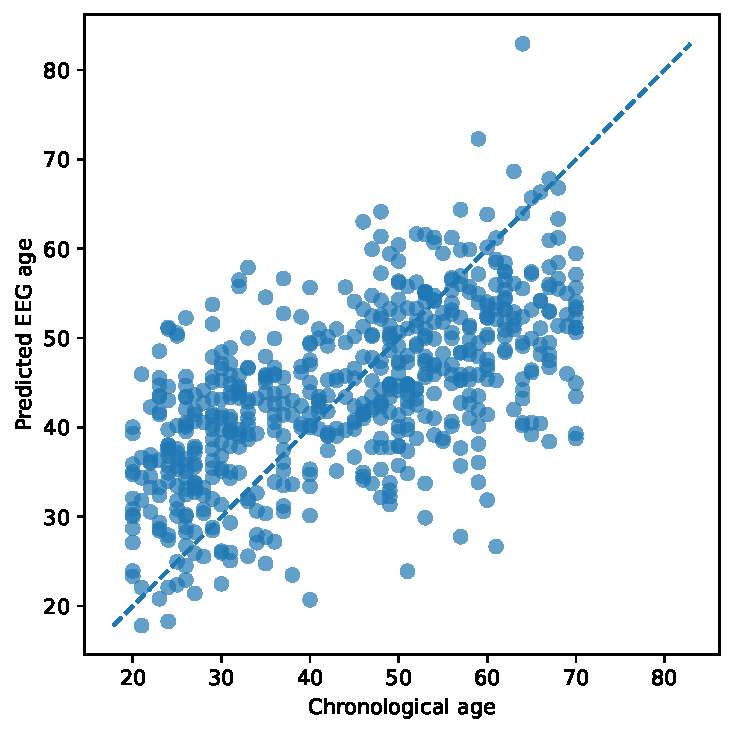
\includegraphics[width=\linewidth]{fig1_brain_age_prediction.pdf}
\caption{Chronological age versus predicted EEG age.}
\label{fig:brainage}
\end{figure}

\subsection{Low-Dimensional EEG Aging Space}

The first ten PCA components explained 91.68\% of EEG feature variance. Explained variance was 34.92\% for PC1, 22.70\% for PC2, 12.46\% for PC3, and 8.53\% for PC4. The most age-associated principal component was PC4 ($\rho=-0.316$, $p=1.54\times10^{-15}$), followed by PC1 ($\rho=-0.271$, $p=9.82\times10^{-12}$). A two-dimensional trajectory defined in the PC1--PC4 plane was significantly associated with chronological age ($\rho=0.344$, $p=2.73\times10^{-18}$), whereas trajectory deviation was not significantly associated with age ($\rho=-0.053$, $p=0.190$).

\begin{figure}[!t]
\centering
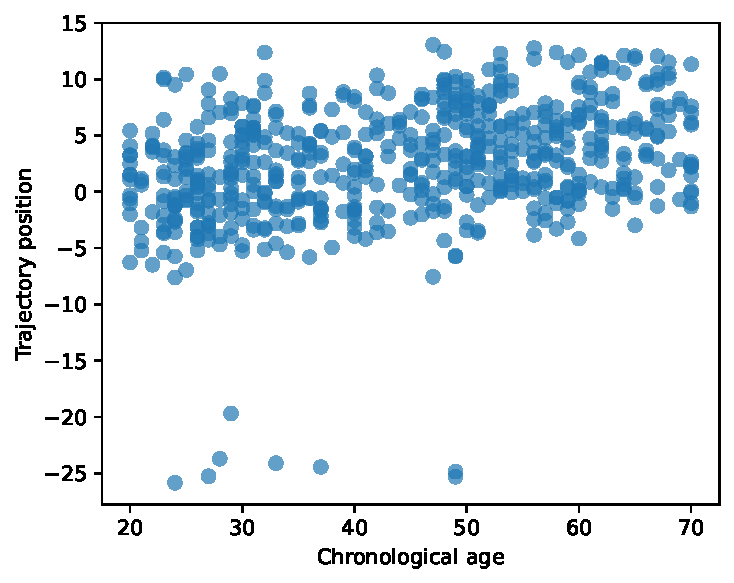
\includegraphics[width=\linewidth]{fig2_age_vs_trajectory_position.pdf}
\caption{Chronological age versus EEG trajectory position.}
\label{fig:trajectory_age}
\end{figure}

\subsection{Test--Retest Stability}

Among 208 longitudinal participants, EEG spectral features showed strong test--retest stability. Mean test--retest Spearman correlation across EEG features was 0.692. The most stable features included global beta/alpha ratio ($\rho=0.894$), occipital relative alpha ($\rho=0.859$), occipital relative low-alpha ($\rho=0.842$), occipital absolute alpha ($\rho=0.837$), and parietal relative alpha ($\rho=0.831$). Stable features were concentrated in alpha-band measures and alpha-normalized ratios.

\begin{figure}[!t]
\centering
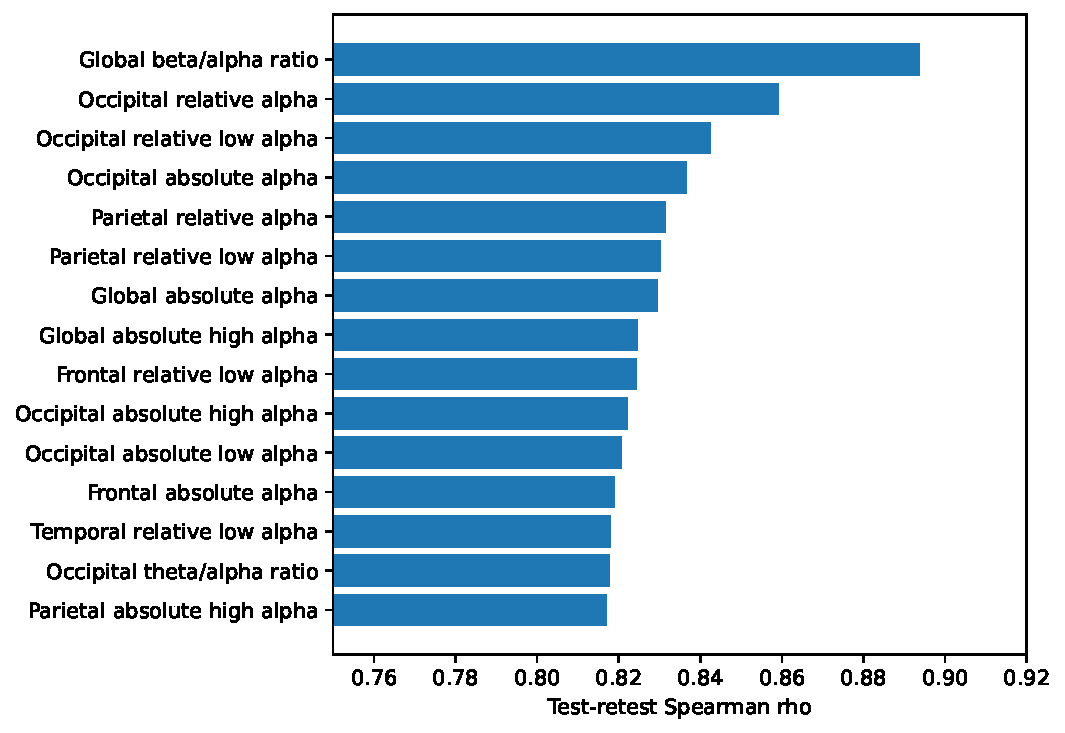
\includegraphics[width=\linewidth]{fig3_test_retest_stability.pdf}
\caption{Test--retest stability of the most stable EEG spectral features after excluding metadata variables. Labels use anatomical and spectral terminology rather than code-level feature names.}
\label{fig:stability}
\end{figure}

\subsection{Longitudinal Movement Along the EEG Aging Trajectory}

The longitudinal subset moved significantly forward along the inferred EEG aging trajectory. Mean trajectory-position change was $\Delta T=0.403$, median $\Delta T=0.522$, and Wilcoxon signed-rank test yielded $p=0.0020$. In contrast, orthogonal trajectory deviation did not significantly change over time, with mean $\Delta D=0.059$, median $\Delta D=0.161$, and $p=0.622$. The longitudinal signal was therefore expressed as movement along the aging axis rather than increased dispersion away from that axis.

\begin{figure}[!t]
\centering
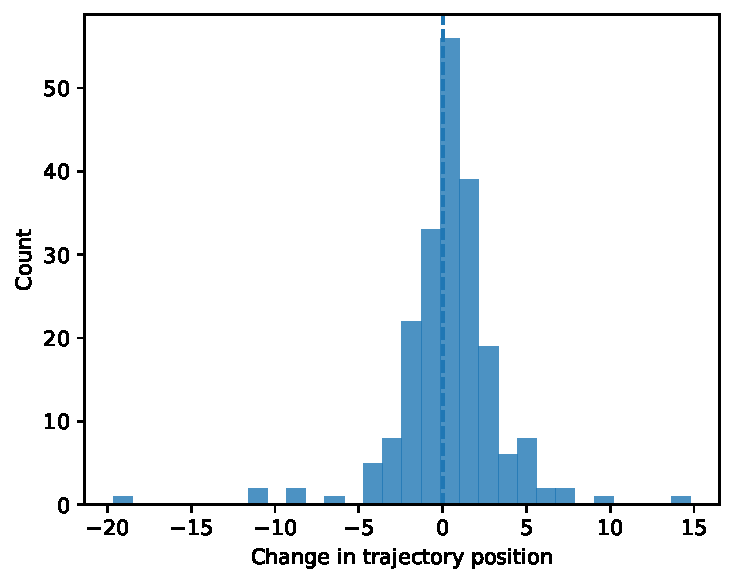
\includegraphics[width=\linewidth]{fig4_longitudinal_shift_distribution.pdf}
\caption{Distribution of longitudinal change in EEG trajectory position.}
\label{fig:shift}
\end{figure}

\subsection{Baseline Trajectory Position Predicts Future Change}

Baseline trajectory position predicted future trajectory change ($\rho=-0.280$, $p=4.09\times10^{-5}$). Participants located farther along the aging manifold at baseline showed smaller subsequent forward shifts. Chronological age did not predict future trajectory change ($\rho=-0.018$, $p=0.795$). Thus, the EEG trajectory coordinate captured prospective electrophysiological dynamics not explained by chronological age.

\begin{figure}[!t]
\centering
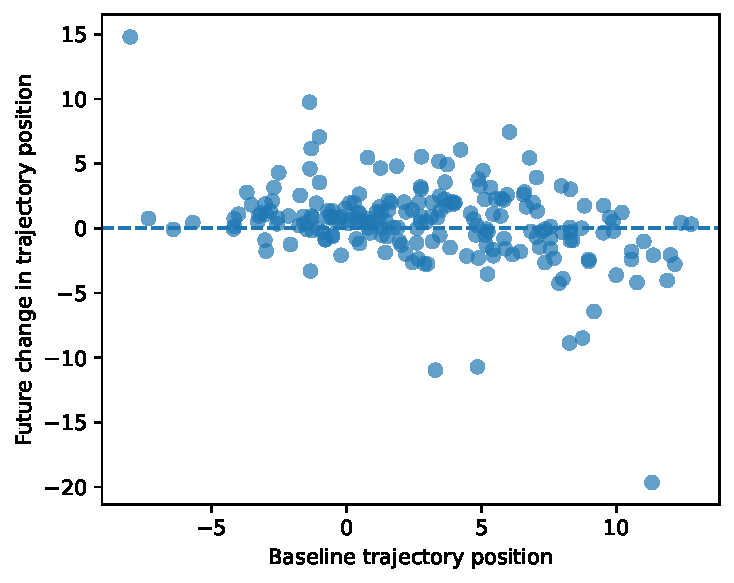
\includegraphics[width=\linewidth]{fig5_baseline_position_vs_future_change.pdf}
\caption{Baseline trajectory position versus future change in trajectory position.}
\label{fig:baseline_future}
\end{figure}

\begin{figure}[!t]
\centering
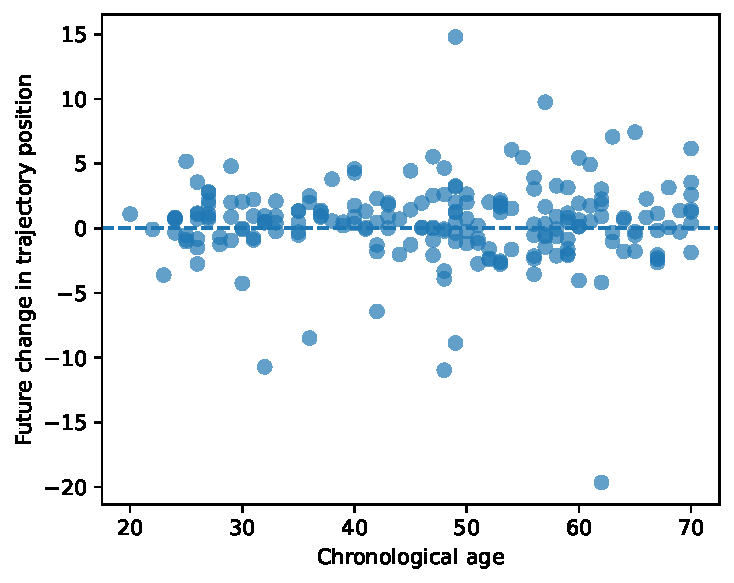
\includegraphics[width=\linewidth]{fig6_age_vs_future_change.pdf}
\caption{Chronological age versus future change in trajectory position.}
\label{fig:age_future}
\end{figure}

\section{Discussion}

This study identifies a longitudinal EEG aging manifold from resting-state spectral features across the adult lifespan. Four findings establish the value of this representation. First, baseline EEG spectral features predicted chronological age with MAE = 9.46 years and correlation $r=0.611$. Second, age-associated EEG variation was organized in a low-dimensional latent space, with a trajectory coordinate significantly associated with age. Third, the longitudinal subset moved significantly forward along this trajectory while remaining stable in orthogonal deviation. Fourth, baseline trajectory position predicted future movement along the manifold, whereas chronological age did not. This pattern indicates structured progression along a normative electrophysiological aging axis rather than nonspecific recording variability.

The spectral signature of aging was biologically coherent. Relative beta power increased with age, whereas high-alpha power decreased. Alpha rhythms are among the most reproducible features of resting EEG and are strongly linked to thalamocortical and cortico-cortical dynamics \cite{klimesch1999eeg,haegens2014alpha,mierau2017state,nunez2006electric}. Age-related changes in alpha activity, broadband spectral structure, and aperiodic electrophysiological activity have been repeatedly associated with adult aging \cite{dustman1993eeg,voytek2015age,donoghue2020parameterizing,gao2017inferring,he2010temporal}. The present results extend this literature by showing that these spectral features form a multivariate trajectory with longitudinal validity.

The distinction between trajectory position and trajectory deviation is central. Trajectory position captures movement along the inferred aging axis. Deviation captures displacement away from that axis. Longitudinally, position increased significantly, whereas deviation did not. This dissociation supports the interpretation that follow-up change reflects progression along a normative aging manifold, not random drift away from the manifold.

The most informative result was that baseline trajectory position predicted future trajectory change while chronological age did not. This establishes that the EEG trajectory coordinate contains prospective information not reducible to calendar age. Participants already farther along the trajectory changed less over follow-up, consistent with convergence toward a bounded electrophysiological aging manifold. This behavior resembles a dynamical system in which the state coordinate carries information about subsequent evolution.

These findings also clarify the role of brain-age prediction. The ridge model achieved the strongest scalar age prediction, but the PCA and PLS latent models provided interpretability by revealing the geometry of aging-related spectral change. The brain-age model and the trajectory model therefore serve different purposes: the former estimates age, whereas the latter describes how EEG states are organized and how they change longitudinally.

Several methodological boundaries define the interpretation of the present results. The analysis used one public EEG dataset, eyes-closed resting-state recordings, and scalp-level spectral summaries rather than source-localized neural generators. Longitudinal age metadata did not vary across sessions in the available participant table, so the longitudinal analysis quantified electrophysiological trajectory displacement rather than estimating change per chronological year. External cohort replication and source-resolved modeling are direct extensions of the present framework.

\section{Conclusion}

Resting-state EEG contains a stable, low-dimensional aging manifold. Baseline spectral features predict chronological age, and longitudinal recordings show significant forward movement along the inferred aging trajectory without increased orthogonal deviation. Baseline trajectory position predicts future trajectory movement, whereas chronological age does not. This establishes EEG trajectory position as a prospective electrophysiological marker of adult brain aging.

\section*{Data Availability}

The EEG data analyzed in this study are publicly available from OpenNeuro as dataset ds005385, version 1.0.3, with DOI 10.18112/openneuro.ds005385.v1.0.3 \cite{openneuro_ds005385}. The dataset descriptor is available in \textit{Scientific Data} \cite{getzmann2024resting}. Derived feature tables and summary statistics will be deposited with the analysis code or released as supplementary material where journal policy permits.

\section*{Code Availability}

The analysis code, including EEG feature extraction, model fitting, trajectory projection, longitudinal analyses, and figure generation, is available at \url{https://github.com/squareshorts/eeg-aging-manifold}.

\section*{Acknowledgment}

The author acknowledges the contributors of OpenNeuro dataset ds005385 and the Scientific Data descriptor describing the Dortmund Vital Study resting-state EEG resource.

\section*{Funding Information}

This work was financially supported by the Conselho Nacional de Desenvolvimento Cient\'ifico e Tecnol\'ogico (CNPq) under Grant No.~309589/2023-1 to A.P., and by the Coordena\c{c}\~ao de Aperfei\c{c}oamento de Pessoal de N\'ivel Superior (CAPES).

\bibliographystyle{IEEEtran}
\bibliography{references}

\end{document}
